After describing different approaches to compute PESs and pointing out why the Dyson orbital formalism combined with a finite element method used to calculate the photoelectron function is well-suited for our needs, in this chapter now
the protocol as being used to obtain the PESs will be presented.\\
In the first section, the computation of the initial (unionised) and final (ionised) states will be described.
Thereafter, in section \ref{sec:grid} the setup of the finite element system used to compute the free electron function as well as the dipole matrix element will be described.
In the final section, the computation of Dyson orbitals will be sketched and it will be described how to transfer it to the finite element setup.

\section{Bound State Functions}
The formalism as it was described in \ref{ch:do} can be used with any quantum chemical method that is able to calculate ground and excited state wave functions and respective energies.
Since density functional theory (DFT) and its time dependent counterpart TDDFT have shown to be accurate and numerically cheap methods, we use these methods here.

In this work the calculations are done using a locally modified version of the program package \prog{NWChem} \cite{nwchem} where a more verbose output enables the reconstruction of all molecular orbitals and thus the computation of the DOs.

\subsection{Ground State Density}
It is based on the Hohenberg-Kohn theorem \cite{HohenbergKohn} which states that the ground-state electron density determines the potential in the SE uniquely and with this also the wave-function.
Thus, the electron density contains all information about a given system.
Since it does not point to a way how to determine the electron density without knowing the wave-function, usually the Kohn-Sham scheme \cite{KohnSham} is used where the electrons are described non-interacting particles in a respective pseudo-potential that is made such that the electron density of these Kohn-Sham orbitals corresponds to the real electron density.
Since the particles do not interact with each other, the Kohn-Sham orbitals $\Psi_j(\vec{r})$ are solutions to the partial differential equation
\begin{equation}
\left( -\frac 12  \nabla^2 + V_\text{eff}(\vec{r}) \right) \Psi_j(\vec{r})=\epsilon_j \Psi_j(\vec{r})
\end{equation}
where $\epsilon_j$ is the binding energy of the respective electron and the effective potential 
\begin{equation}
V_\text{eff}(\vec{r})=V_\text{ext}(\vec{r})+ \int \frac{\rho(\vec{r}')}{|\vec{r}-\vec{r}'|} d\vec{r}' + V_\text{xc}(\vec{r})
\end{equation}
can be separated into the external potential $V_\text{ext}(\vec{r})$ which consists of the attractive nuclear electrostatic potential.
The second term is the electrostatic interaction of the electrons. 
With these contributions, this formalism is on the level of theory of the Hartree-theory, missing the exchange and correlation.
The respective contributions are approximated by $V_\text{xc}(\vec{r})$ together with the error in kinetic energy to accound for the fact that the single-electron functions of the Kohn-Sham scheme differ from the real electrons and thus have an other kinetic energy as well \cite{Holthausen}.

Assuming that the Kohn-Sham orbitals coincide with the physical orbitals, which is known to be not the case, the exchange potential acts on an orbital $\Psi_i(\vec{r})$ as
\begin{equation}
V_{x;j}(\vec{r})\Psi_i(\vec{r}) =\int \Psi_j^\dagger(\vec{r}')\frac{1}{\left|\vec{r}-\vec{r'}\right|} \Psi_i(\vec{r}') d\vec{r}' \Psi_j(\vec{r})
\end{equation}
and thus is non-local \cite{Holthausen}, the ``exact'' exchange energy thus corresponds the term $E_{x}=\sum_{i<j}\int \Psi_i^\dagger(\vec{r}) V_{x;j}(\vec{r}) \Psi_i(\vec{r}) d\vec{r}$  respectively.
In DFT usually the exchange energy is approximated as a local functional of the density and its derivative, leading to the so-called local density approximation and gradient corrected functionals.
The Becke \cite{blyp} exchange-functional used in this work has the form
\begin{equation} \label{eq:blypXC}
E_x=\frac 32 \left(\frac{3}{4\pi}\right)^\frac 13 \sum_\sigma \int \rho_\sigma(\vec{r})^\frac 43 d^3\vec{r} 
-\beta \sum_\sigma \int \rho(\vec{r})^\frac 43 \frac{x_\sigma(\vec{r})^2}{1+6\beta x_\sigma \text{sinh}^{-1}( x_\sigma (\vec{r}))} d^3\vec{r}
\end{equation}
where $\sigma$ denotes the spin polarisations and $x_\sigma(\vec{r})=\frac{|\nabla \rho_\sigma(\vec{r})|}{\rho_\sigma^\frac 43}$, the first term is corresponds to the local density approximation and the second one is a semi-empirical gradient correction which is constructed such that the asymtotic behaviour of the exchange energy and electron density
\begin{align}
  \lim_{r\rightarrow\infty} E_x^\sigma(\vec{r}) & =-\frac{1}{|\vec{r}|} \\
  \lim_{r\rightarrow\infty} \rho(\vec{r}) & =e^{-a_\sigma |\vec{r}|}
\end{align}
with $a_\sigma$ is a constant related to the ionisation potential of the system under study \cite{blyp}.
The prefactor of the gradient correction, $\beta$, was determined by fitting to several atomic noble-gas systems and is set to be $\beta=0.0042$ in atomic units \cite{blyp}.

Finally, the correlation energy is defined as the difference between the sum of the previously discussed terms and the correct energy.
The correlation potential is defined as the functional derivative of the correlation energy respectively $V_c(\vec{r})=\frac{\partial E_c[\rho]}{\partial\rho(\vec{r})}$.
In the case of the
The LYP-correlation energy functional is based on the Colle-Salvetti formula which estimates the correlation energy in the Hartree-Fock approach and introduces two parameters that are set by fitting to experimental data \cite{lyp}.

\subsection{Excited State Properties}
The DFT is not only a well-established method to obtain ground-state properties of many different kinds of systems, but it has also a time-dependent counterpart, formally based on the Runge-Gro\ss theorem \cite{RungeGross}.
Commonly, when referring to time-dependent DFT (TDDFT), the linear-response TDDFT is meant \cite{dreuw}.
It constitutes a first order perturbation expansion and can be used to obtain the enegies and occupations of excited states using the so-called Casida-equation \cite{casida}
\begin{equation} \label{eq:casida}
\begin{bmatrix} \mat{A} & \mat{B} \\ \mat{B}^\dagger & \mat{A}^\dagger\end{bmatrix}
\begin{bmatrix} \vec{X} \\ \vec{Y} \end{bmatrix} =
\omega \begin{bmatrix} \mat{1} & \mat{0} \\ \mat{0} & -\mat{1}\end{bmatrix}
\begin{bmatrix} \vec{X} \\ \vec{Y} \end{bmatrix}
\end{equation}
where 
\begin{align}
\mat{A}_{ia,jb}& =\delta_{ij}\delta_{ab}(\varepsilon_a-\varepsilon_i)+ 
\int \int d\vec{r} d\vec{r}'\left( \Psi_i(\vec{r}) \Psi_a(\vec{r})  \Psi_j(\vec{r}') \Psi_b(\vec{r}') 
\Psi_i(\vec{r}) \Psi_j(\vec{r}) \Psi_a(\vec{r}') \Psi_b(\vec{r}') \frac{1}{|\vec{r}-\vec{r}'|}  \right) ,\\
\mat{B}_{ia,jb}& = \int \int d\vec{r} d\vec{r}'\left( \Psi_i(\vec{r}) \Psi_a(\vec{r})  \Psi_b(\vec{r}') \Psi_j(\vec{r}') 
\Psi_i(\vec{r}) \Psi_b(\vec{r})  \Psi_a(\vec{r}') \Psi_j(\vec{r}') \frac{1}{|\vec{r}-\vec{r}'|}  \right) 
\end{align}
and $\mat{1}$ is the unity matrix.
The indices $i,j$ and $a,b$ denote occupied and virtual orbitals with binding energy $\varepsilon_i, \varepsilon_a$ respectively \cite{dreuw}.
The Casida equation (\ref{eq:casida}) is an non-hermitian eigenvalue problem whose eigenvalues $\omega$ correspond to the transition energies and the eigenvectors denote the transition coefficients.
The lower half of the eigen vector, denoted as $\vec{Y}$, corresponds to negative excitation energies $\varepsilon_i$ and can be assigned to de-excitations from virtual orbitals which makes no physical sense if the reference state is a ground state \cite{dreuw}.
Since the matrix $\mat{B}$ contains usually only small elements, it is often set to zero.
This is called Tamm-Dancoff approximation and reduces the original equation to a hermitian equation of half dimensionality \cite{casida}.

\subsection{OTRSH-scheme}
One main issue concerned with the DFT-formalism is that the approximate exchange functional decays exponentially instead of $\frac 1r$ and $\frac{1}{r^4}$ for the exchange and correlation terms respectively.
This wrong behaviour affects the obtained wave functions and thus the orbital energies \cite{Bokareva}.

To reduce this error, so-called range-separated hybrid (RSH) functonals are used, in which the DFT-exchange term is used for small interelectronic distances only, while at larger distances, where correlation effects are not that important, the Hartree-Fock excact-exchange is used.
The interchange between the schemes is done by the separation
\begin{equation}
   \frac 1r = \frac{\alpha +\beta erf(\omega r)}{r} +\frac{1-\alpha-\beta erf(\omega r)}{r}
\end{equation}
where $\alpha+\beta=1$ and $\beta$ are parameters to be chosen.
Besides taking the standard parameters, an ab-initio scheme to chose them is the optimally-tuned RSH (OTRSH) scheme where the functional
\begin{equation}\label{eq:J_ao}
   J(\alpha_\text{opt},\omega_\text{opt})=min_{\alpha, \omega} \left\{ |E_N(\alpha,\omega)-E_{N-1}(\alpha,\omega)-\varepsilon_\text{HOMO}| \right\}
\end{equation}
is minimised, making sure that Koopman's theorem is fulfilled \cite{Bokareva}.
Besides similar functionals which account for the electron affinities or ionisation potentials of lower-lying orbitals, the optimisation can be done according to stability or derivative discontinuity.
\textcolor{blue}{the most-straight line of partial charges} can be chosen as equivalent ab-initio criteria.
\textcolor{red}{More details on these schemes? Not mention them at all?}

For this optimization procedure the Gaussian package \prog{G09} \cite{g09} is used with the 6-31G(d) \cite{6-31g,6-31gd} basis set and the functional LC-BLYP \cite{lcblyp}. 
The ground state DFT calculation, determination of geometries and the linear-response TDDFT calculations have been conducted with a locally modified version of \prog{NWChem} \cite{nwchem}, employing the basis set def2-tzvp \cite{def2tzvp} without symmetry restrictions.
The Kohn-Sham orbitals (obtained by ground state DFT) and CI-coefficients (obtained by linear-response TDDFT which yields the configuration interaction singles expansion for a number of excited states) as well as the atomic overlap matrix are interfaced to the in-house software \prog{DYSON} \cite{MAgg} that computes the DOs.
The integration of the overlap matrix in eq. (\ref{eq:DO}) finally is perfomed using \prog{ezDyson} \cite{ezDyson}.

\subsection{Computing the Dyson orbital}
The DO is computed in the framework of this thesis with the in-house code \prog{DYSON} \cite{MAgg}.
%Considering a state as linear combination of CI-states is denoted as weak-coupling representation \cite{McCarthy}.

\section{Free electron function}
The FEF is computed with a finite element scheme, using the program \prog{Free Willy} developed in the framework of this thesis.
It is based on the library \prog{Libmesh} \cite{libmesh} which itself uses sevaral libraries for the required linear algebra and the mesh-setup.

\subsection{Setup of the Grid}
\label{sec:grid}
The most crucial part of the FEM is the mesh under usage. 
In the program \prog{FreeWilly} it is obtained from a set of points via Delaunay triangulation (see \ref{app:delaunay} for details) using the library \prog{tetgen} \cite{tetgen}.
The distribution of these points is responsible for the quality of the obtaind solution and depends on many parameters in a non-trivial way.
The dependence is in particular on
\begin{description}
   \item[The molecular geometry] Close to the cores it should be denser, at larger distances a coarser grid is possible.
   \item[The kinetic energy] of the photo electron which gives the maximum distance between two points
   \item[The largest angular momentum of the Dyson orbital] determines the angular momentum of the photoelectron to be resembled.
\end{description}

In the general scheme the generation of the point-distribution follows the suggestion of Son and Chu \cite{Son_Chu}:
The grid is set up of atomar grids, \textit{e.g.} spherical distributions, each centered at atoms where the overlapping regions are cut off.
The radii of these spheres needs to be much larger than the bond lengthes, holes or interatomic gaps in the molecule to (\textit{e.g.} holes in aromatic rings or the space between ligands of larger molecules).
Using this scheme, the grid-parameters are determined by the size of the larges box $r_\text{max}$, number $N$ of spheres used as well as the radial distribution of them and the angular distribution of points on these spheres.
\begin{figure}
   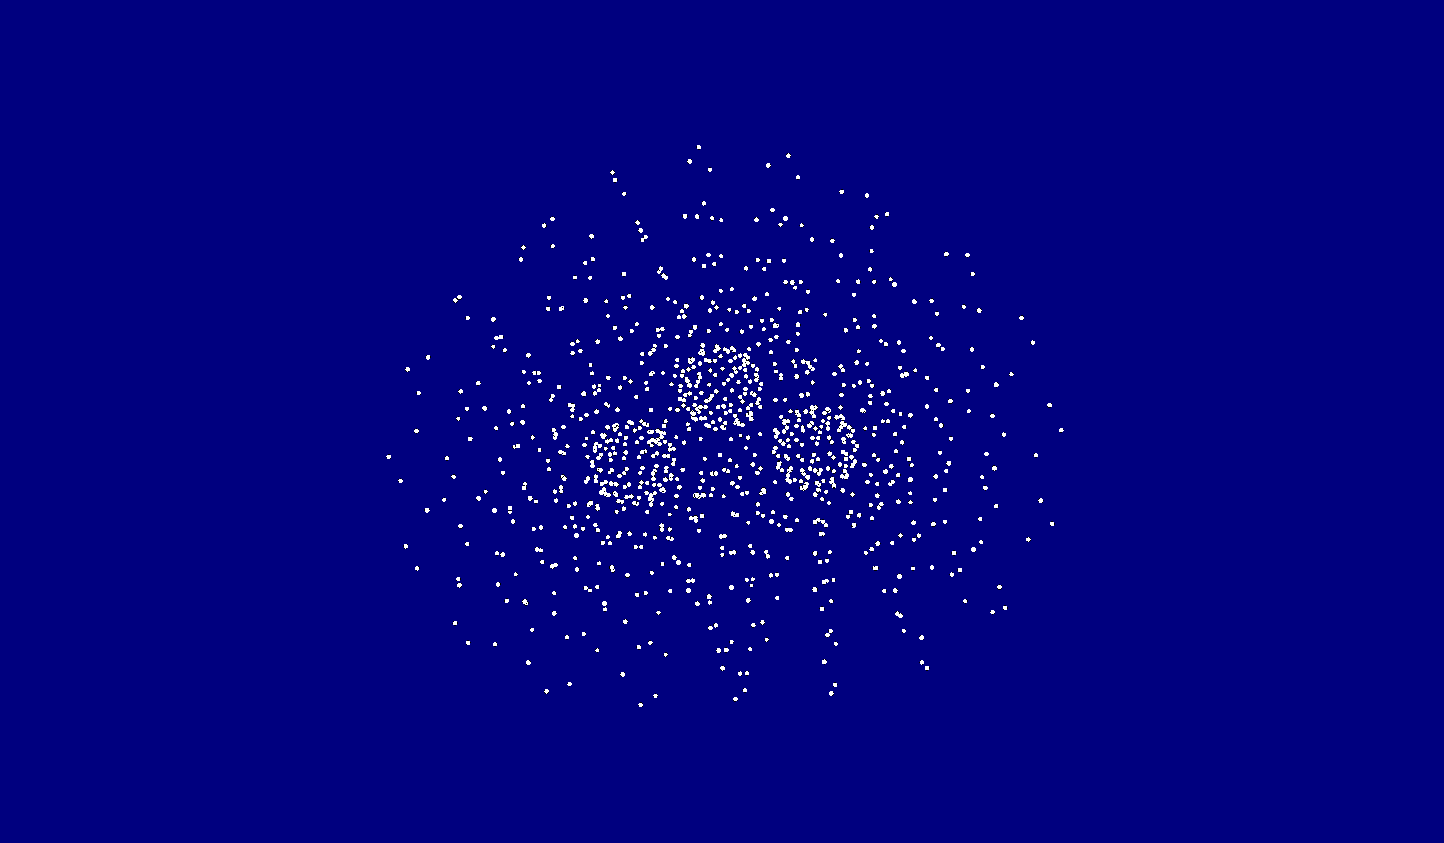
\includegraphics[width=0.5\textwidth]{water1}
   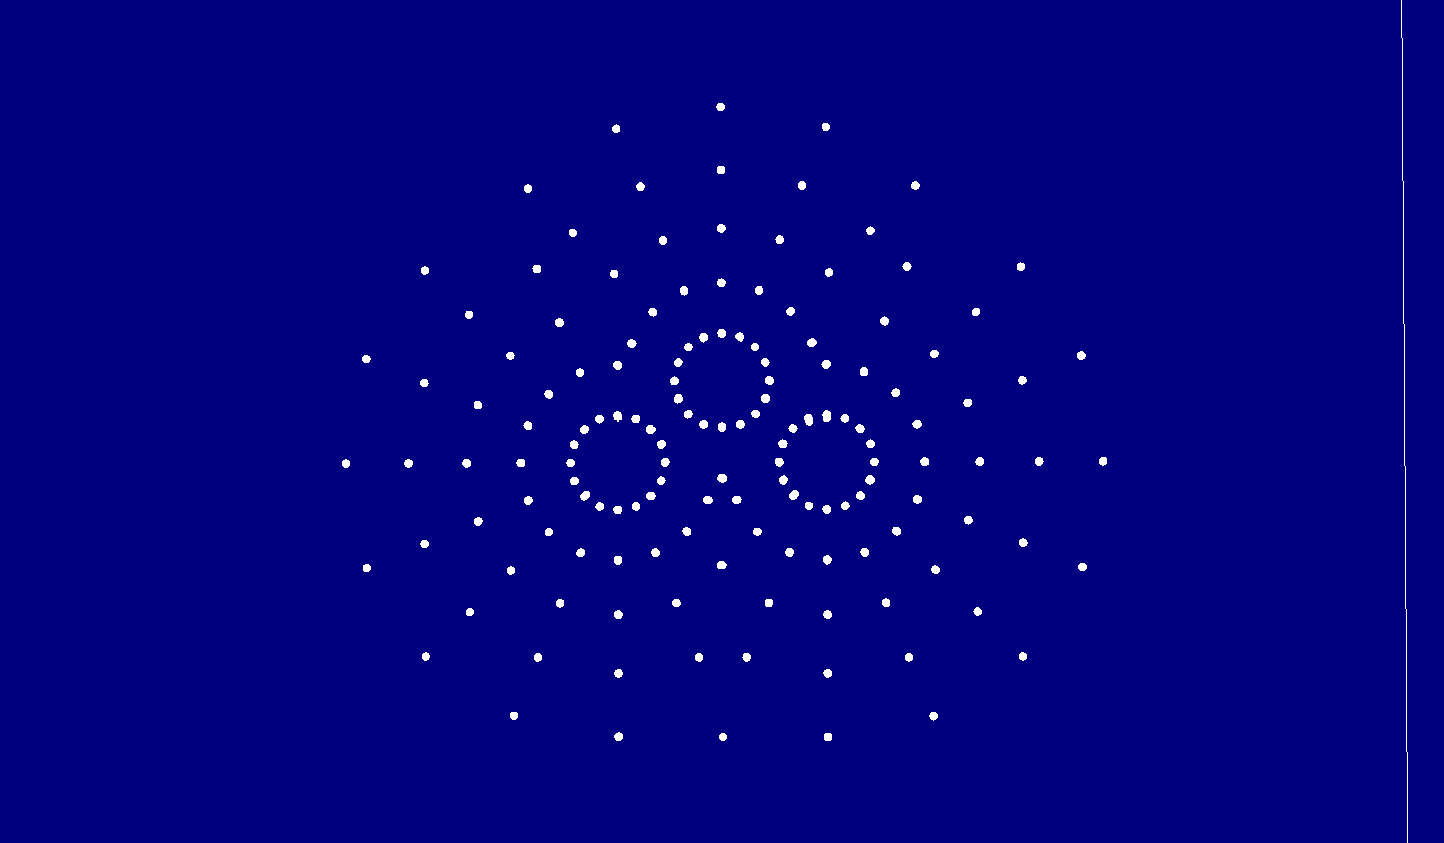
\includegraphics[width=0.5\textwidth]{water2}
   \caption{Example of a mesh for the water-geometry. It consists of $5$ spheres with constant number of points per sphere. The overlapping regions are cut off. Left: cut through the nuclear plane.}
   \label{fig:molmesh}
\end{figure}

For the radial distribution Son and Chu \cite{Son_Chu0} suggested the scheme
\begin{equation}
r_i=\frac{il}{N-i+\frac{lN}{r_\text{max}}} \qquad i=1,\hdots ,N 
\end{equation}
where $l$ is a parameter to chose.
As an alternative distribution, here the formula
\begin{equation}
r_i=\frac{il}{\left( \frac Ni \right)^p \left(\frac{Nl}{r_\text{max}}-1\right) +1} \qquad i=1,\hdots ,N 
\end{equation}
is to be tested where $l$ and $p\geq 1$ are parameters to chose whereby the condition $N<\frac{r_\text{max}}{l}$ should be fulfilled to prevent the singularity.
%Thereby it is important to mention that in this scheme (in contrast to the above one) the (asymptotic for $r\rightarrow \infty$) maximum distance between two spheres is $l$ and hence could be physically chosen to $l\approx \frac \lambda 2$.

While the distribution of spheres follows, at least on a qualitative level, a clear scheme since it should always resemble the local kinetic energy, the distribution on the surface of each sphere is not that clear.
Qualitatively it is preferable to chose a regular grid but this more challenging.
Since the ... grid, which is known from the ... is clearly a bad choise due to its high density close to the poles, in geological applications often so-called geodesic grids are chosen.

\textcolor{red}{
Some explanations are given here:\\ %https://www.maths.unsw.edu.au/about/distributing-points-sphere
- Lebedev-grid -> try to get spherical harmonics with highest L accurate.\\
-If also required: all weights should be equal: spherical t-designs. \\
Leads directly to the question of uniform distribution.-> not directly by algorithms\\
- other approach: close packings \\
- energy minimisation: Consider nodes as interacting particles -> minimise E for some model potential.\\
see} \textcolor{blue}{http://people.maths.ox.ac.uk/beentjes/Essays/QuadratureSphere.pdf}.
\textcolor{green}{
- crude but fast algorithms
Since in finite element theory the sphere neither needs to be really round nor is there any global functional defined on it,
the complicated distributions described above may be not even needed. 
An other approach therefore is to use an algorithm that gives just a more or less uniform distribution.}

Approach used for climate models: so-called geodesic grids: subdivision of polyhedra, projected onto the sphere\cite{geodesic1, geodesic2}, see also
%http://kiwi.atmos.colostate.edu/BUGS/geodesic/
%http://kiwi.atmos.colostate.edu/BUGS/pdf/ZM-grid.pdf
%http://kiwi.atmos.colostate.edu/BUGS/pdf/conservation.pdf
%http://kiwi.atmos.colostate.edu/BUGS/pdf/ccsr.pdf
for further information.

The point sets I took are from here: %http://web.maths.unsw.edu.au/~rsw/Sphere
\cite{womersley,fliegeMaier}.

The above mentioned techniques show the large variety of different approaches and it is not very clear which one will meet our needs best.
Moreover, here the problem is not only two dimensional but the whole sphere (not only its surface) needs to be subdivided. 
Hence, besides the question of a radial density of different spherical surfaces, also the number of points per sphere as function of the radial distance 
needs to be considered.

Whether the approach of subdividing the atomic meshes into radial and angular parts as opposed to another volume tessellation can be questioned and 
may turn out to be inefficient.
Application of Geodesic grid in calculating surface charges: \cite{geodes_charge}, also mentioning Connolly algorithm (refs 26, 29 therein).

The second scheme has a divergence around $Nl=r_\text{max}$. 
It can be shown that the condition $N\leq \frac rl $ is enough here to stabilise it.

\textcolor{yellow}{
If the above described procedures prove to be too inefficient, one could try to implement some WKB-based scheme similar to \cite{impLDVR} but in 3D.
Thereby, the number of points in a given volume element is determined by $N_i=\frac{\alpha_i}{\alpha} N$ where $\alpha=\sum_i \alpha_i $ and
\[ \alpha_i= \int_V dV \sqrt{2\mu (E-V(r))} \]
.This ensures dense points there, where the potential is lowest and a coarse mesh far away; however, a consistent formulation in 3D would need to be invented.
}

To account for the molecular geometry and the general tendency of the photo electron to oscillate stronger in the vicinity of the nuclei, the mesh is built out of spheres, centred at the nuclear positions.
Thereby, a study of Son \cite{Son_Chu0} had shown that it is numerically most efficient when the overlapping regions of these spheres are cut out.
Figure \ref{fig:molmesh} shows an example for the water molecule.\\
For the radial distribution we will use the the function
\[
r_i = \frac{1+x_i}{1-x_i+\frac{2L}{r_{max}}} L \qquad x_i = \frac{2i}{N_r} -1
\]
suggested by Son \textit{et. al.}\cite{Son_Chu0, Son_Chu}.
The parameters $N_r$, $L$ specifying the number of spheres and their distribution; the larger $L$ is, the denser are the spheres close to the centre.\\
The optimal choise of these parameters as well as the angular distribution of points on the spheres is still an open quetion.
Finally, after putting the points together as described above, they are connected to a Delaunay triangulation using \prog{tetgen} \cite{tetgen}. 
Here additional points may be introduced to guarantee well-shaped elements (\texttt{i.e.} no sharp peaks).
\textcolor{red}{
one scheme suggested by Son and Chu \cite{Son_Chu0}:
\[ r_i=\frac{il}{N-i+\frac{lN}{r_\text{max}}} \qquad i=1,\hdots ,N \]
where $l$ is a parameter to chose.
Own scheme:
\[ r_i=\frac{il}{\left( \frac Ni \right)^p \left(\frac{Nl}{r_\text{max}}-1\right) +1} \qquad i=1,\hdots ,N \]
where $l$ and $p\leq 1$ are parameters to chose. Thereby it is important to mention that in this scheme (in contrast to the above one) the (asymptotic for $r\rightarrow \infty$) maximum distance between two spheres is $l$ and hence could be physically chosen to $l\approx \frac \lambda 2$.\\
The second scheme has a divergence around $Nl=r_\text{max}$. 
It can be shown that the condition $N\leq \frac rl $ is enough here to stablilise it. }

Besides the tricky question about this mapping, also the number of points per sphere depending on the radial distance should be considered. 
In \cite{Son_Chu0} this is chosen to be constant without further discussion but of course there are several possible design criteria as well.
Besides a constant number, also a constant spherical density (hence $N\propto r^2$) are possible; However, it might be sensible to follow a similar idea than in the radial mapping: Being fine close to the nuclei and get coarser with increasing distance.
In particular, I followed the design rule of keeping the space between points in radial direction similar to space between points in angular distribution.
Hence, $d_\text{spheric}=\sqrt{\frac{4\pi r_i^2}{N_i}}\approx r_i-r_{i-1}$.
For the above described radial schemes, this results in 
\[
N_i= \frac{4\pi}{ \left(1-\frac{i-1 }{i}\frac{N-i+\frac{lN}{r_\text{max}}}{N-i+1+\frac{lN}{r_\text{max}}}\right)^2 }
\]
for the first scheme and 
\[
N_i= \frac{4\pi}{\left(1-\frac{i-1 }{i}\frac{ (\frac{N}{i})^p \left(\frac{lN}{r_\text{max}}-1\right)+1}{ (\frac{N}{i-1})^p\left( \frac{Nl}{r_\text{max}} -1 \right) +1 } \right)^2 }
\]
for the latter.\\
The respective radii and number of points per sphere are shown in figure \ref{fig:maps}.\\
Special mapping schemes are the constant radial mapping $r_i=a i$ which corresponds to a constant spherical grid density $N_i=4\pi a^2 i^2$ and an exponential map $r_i=q^i r_0$ which would require a constant number of spherical grid points $N_i=\frac{4\pi q^2}{(1-q)^2}$ according to the rule derived above.

\begin{figure}
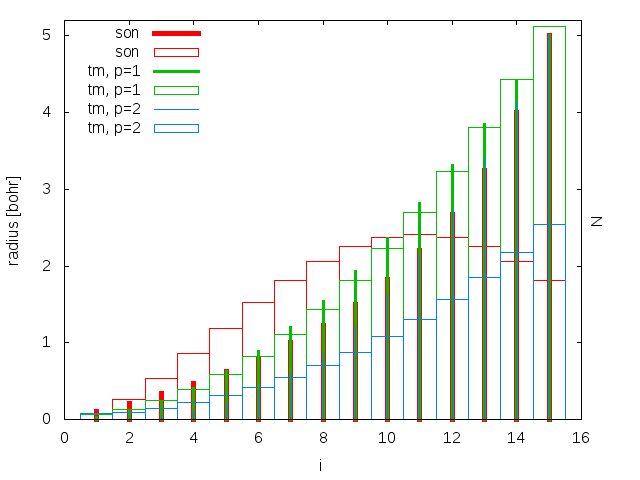
\includegraphics[width=0.7\textwidth]{Figures/RadialMap}
\caption{the radius and number of points of the spheres as for $N=15$, $r_\text{max}=5$ and $l=2$.}
\label{fig:maps}
\end{figure}

Since some of the spherical schemes described above allow only for certain numbers of points each, here, the best approximation is used respectively.

\subsection{Benchmark}
\textcolor{blue}{
Tested on Lithium with a sphere with $r_\text{max}=2.8$
1:  Using the mapping of Son with a naive approach, setting the number of circles by hand and growing quadratically with the size  ($N_\text{circle}=20$, $l= 2.0$ , $N= 10$)
2: using the Son scheme with N according to above formula
3: using the tm scheme as described above, p=1
4: using the tm scheme as described above, p=2}

\begin{tabular}{|c|c|c|}
\hline
scheme & \#elements & error in energy [a.u.]\\
\hline
1      & 2370      & 0.496220, 0.520199, 0.572279 \\
2      & 2022      & 0.038136, 0.046119, 0.055691 \\
3      & 2166      &-0.003638, 0.027219, 0.050588 \\
4      & 2338      & none converged \\
\hline
\end{tabular}
Thereby, the number of elements were kept as similar as possible.

\subsection{Obtaining ESP}
 - obtained from \prog{NWChem}
 - interpolation of that grid

\section{Obtaining the DOs}
 - from coefficients to values
